\documentclass[border=10pt]{standalone}
\usepackage[svgnames]{xcolor}
\usepackage{amsmath}
\usepackage{pgfplots}
\pgfplotsset{compat=newest}
\usepackage[sfdefault]{FiraSans}
\usepackage{FiraMono}
\renewcommand*\familydefault{\sfdefault}
\begin{document}
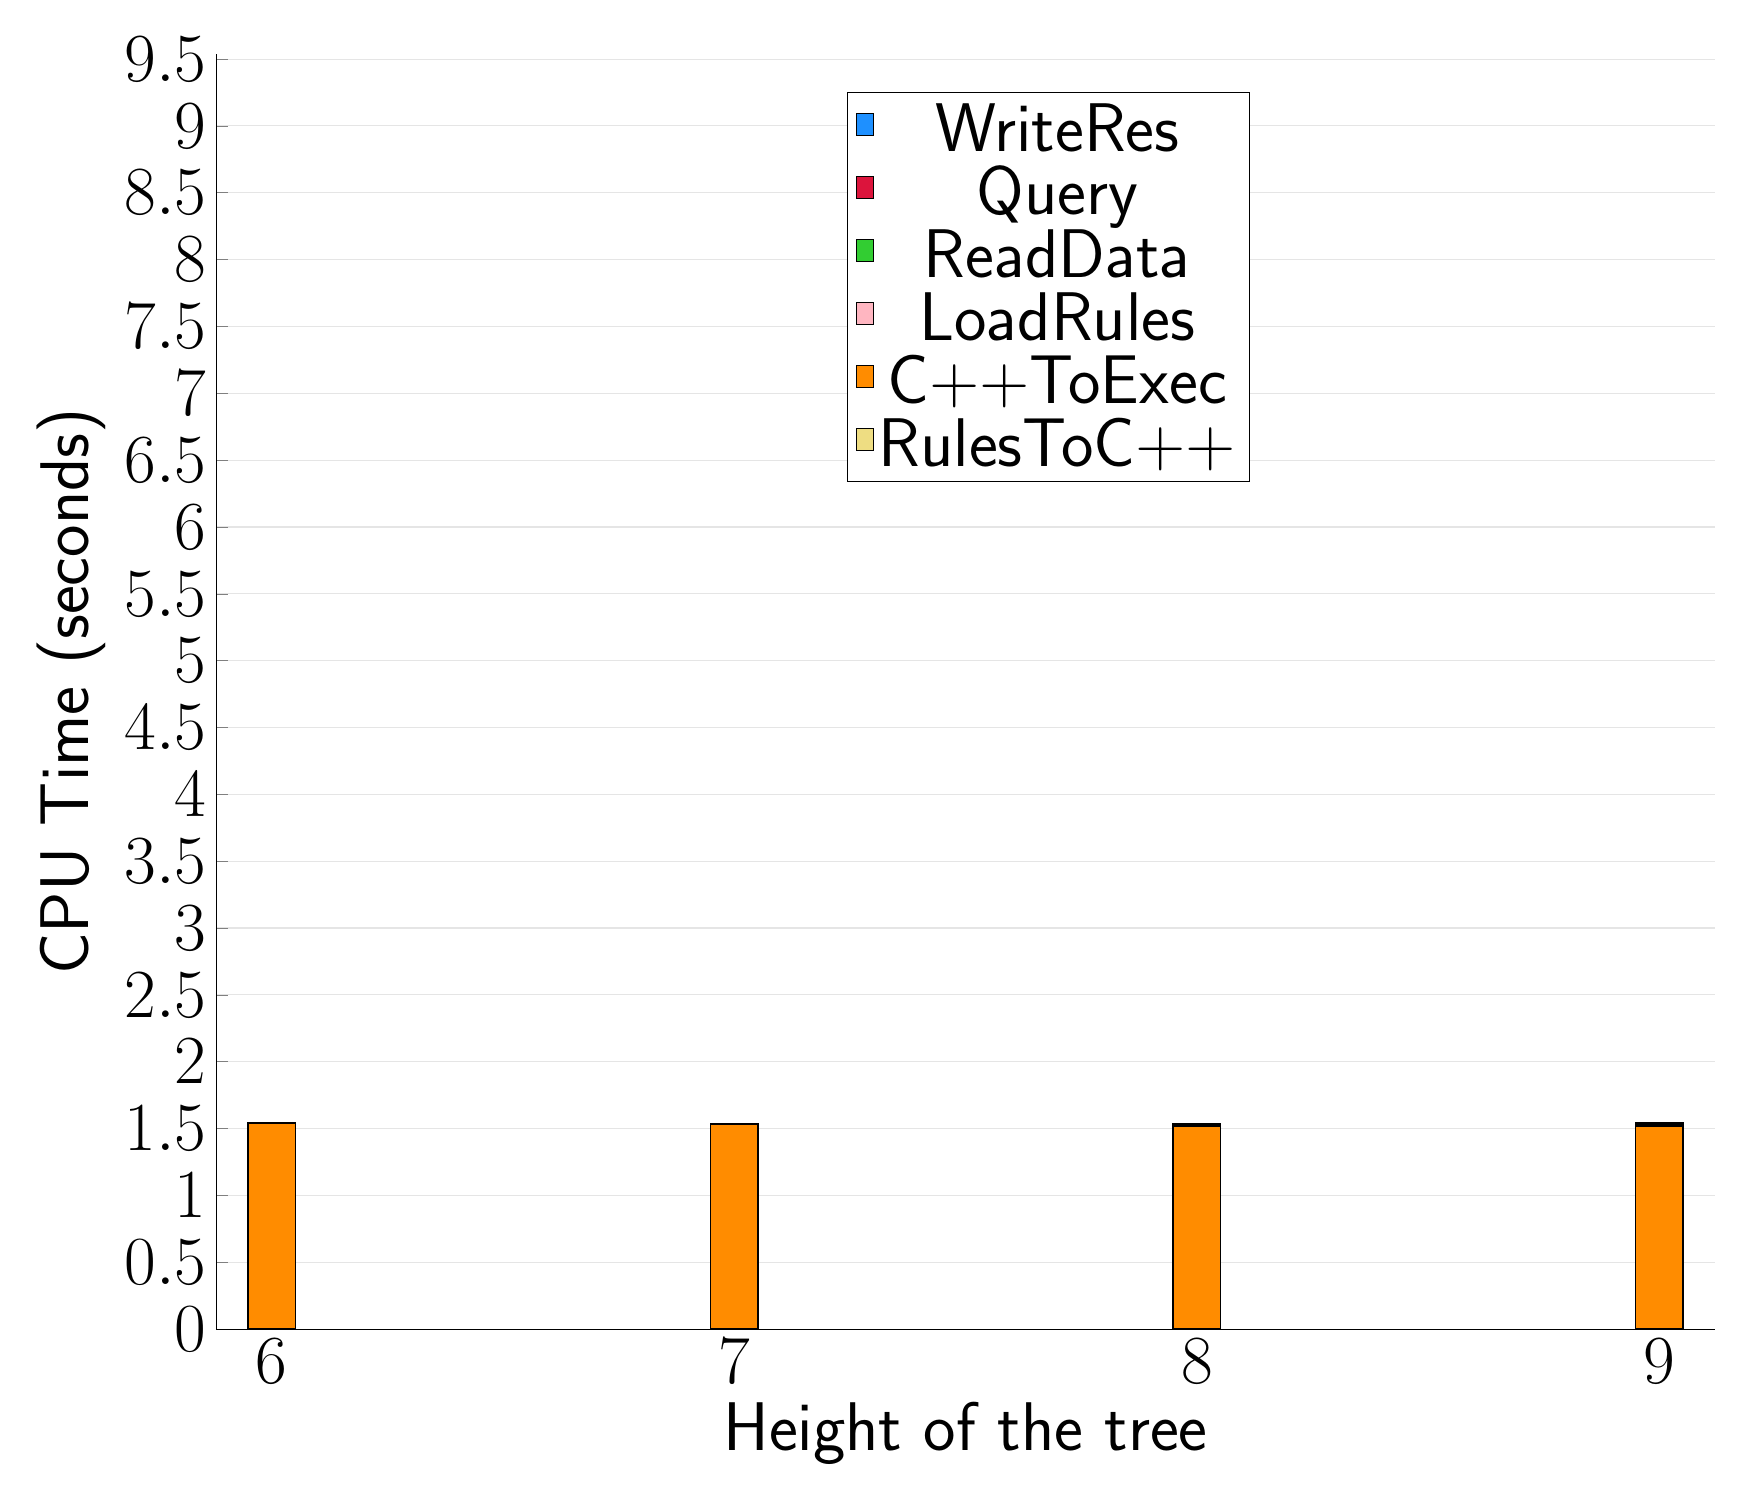
\begin{tikzpicture}
\begin{axis}[
   ybar stacked,
   width=1.7\textwidth,
   bar width=0.6cm,
   ymajorgrids, tick align=inside,
   major grid style={draw=gray!20},
   xtick=data,
   ymin=0, ymax=9.54,
   axis x line*=bottom,
   axis y line*=left,
   enlarge x limits=0.04,
   legend style={
       at={(0.69, 0.97)},
       anchor=north east,
       legend columns=1,
       font=\Huge,
   },
   ylabel={CPU Time (seconds)},
   xlabel={Height of the tree},
   label style={font=\Huge},
   tick label style={font=\Huge},
]
\addlegendimage{fill=DodgerBlue, draw=black, line width=0.2pt}
\addlegendentry{WriteRes}
\addlegendimage{fill=Crimson, draw=black, line width=0.2pt}
\addlegendentry{Query}
\addlegendimage{fill=LimeGreen, draw=black, line width=0.2pt}
\addlegendentry{ReadData}
\addlegendimage{fill=LightPink, draw=black, line width=0.2pt}
\addlegendentry{LoadRules}
\addlegendimage{fill=DarkOrange, draw=black, line width=0.2pt}
\addlegendentry{C++ToExec}
\addlegendimage{fill=LightGoldenrod, draw=black, line width=0.2pt}
\addlegendentry{RulesToC++}
\addplot +[fill=LightGoldenrod, draw=black, line width=0.55pt] coordinates {
(6, 0.0020000000000000005)
(7, 0.0)
(8, 0.0)
(8, 0.0)
(8, 0.0)
(9, 0.0020000000000000005)
(9, 0.0020000000000000005)
(9, 0.0)
(9, 0.0)
(9, 0.0)
};
\addplot +[fill=DarkOrange, draw=black, line width=0.55pt] coordinates {
(6, 1.536)
(7, 1.534)
(8, 1.518)
(8, 1.528)
(8, 1.53)
(9, 1.52)
(9, 1.5180000000000002)
(9, 1.5379999999999998)
(9, 1.5240000000000002)
(9, 1.528)
};
\addplot +[fill=LightPink, draw=black, line width=0.55pt] coordinates {
(6, 0.0001314)
(7, 0.00015080000000000003)
(8, 0.0001406)
(8, 0.00015560000000000001)
(8, 0.00014299999999999998)
(9, 0.000143)
(9, 0.00013300000000000003)
(9, 0.000152)
(9, 0.0001466)
(9, 0.00014399999999999998)
};
\addplot +[fill=LimeGreen, draw=black, line width=0.55pt] coordinates {
(6, 0.0007042000000000001)
(7, 0.00099)
(8, 0.0014394)
(8, 0.0014698)
(8, 0.001486)
(9, 0.0022957999999999998)
(9, 0.0021966)
(9, 0.0022248)
(9, 0.0025182)
(9, 0.0024036)
};
\addplot +[fill=Crimson, draw=black, line width=0.55pt] coordinates {
(6, 0.0005856000000000001)
(7, 0.0014735999999999998)
(8, 0.0032294000000000003)
(8, 0.0032914)
(8, 0.0032984)
(9, 0.006557199999999999)
(9, 0.0064094)
(9, 0.0064446)
(9, 0.006766799999999999)
(9, 0.006919399999999999)
};
\addplot +[fill=DodgerBlue, draw=black, line width=0.55pt] coordinates {
(6, 0.0004122)
(7, 0.0004384)
(8, 0.0004732)
(8, 0.000516)
(8, 0.000541)
(9, 0.0003858)
(9, 0.0004768)
(9, 0.0004224)
(9, 0.0004776)
(9, 0.000432)
};
\end{axis}
\end{tikzpicture}

\end{document}
